% To make the graphics
% tgif -print -epsi wvs-063-diag.obj; epstopdf wvs-063-diag.eps
% tgif -print -jpeg wvs-063-diag.obj
% tgif -print -epsi wvs-063-grids.obj; epstopdf wvs-063-grids.eps
% tgif -print -jpeg wvs-063-grids.obj
% tgif -print -epsi wvs-063-eq-circ.obj; epstopdf wvs-063-eq-circ.eps
% tgif -print -jpeg wvs-063-eq-circ.obj
% tgif -print -epsi wvs-048-grid2.obj; epstopdf wvs-048-grid2.eps
% tgif -print -jpeg wvs-048-grid2.obj

\makeatletter\let\ifGm@compatii\relax\makeatother
\documentclass[landscape]{beamer}
\usepackage[nofancy,notoday]{rcsinfo}
\usepackage{color}
\usepackage{amsmath}
\usepackage{moreverb}
\usepackage{multicol}
\usepackage{graphicx}
\usepackage{floatflt}
%
\renewcommand{\b}{\mathbf}
\renewcommand{\d}{\text{d}}
\newcommand{\T}{^{T}}
\newcommand{\cs}[1]{$_{\text{#1}}$}
\newcommand{\inv}{^{\mathrm -1}}
\newcommand{\cp}[1]{$^{\text{#1}}$}
\newcommand{\degsym}{\ensuremath{^\circ}}
\newcommand{\newframe}[2][]{\begin{frame}\frametitle{\hfill #2 \hfil}}

\parskip 2pt
%
% -----------------------------------------------------------------------------
%
\title{Summary of Full Forward Model}
\subtitle{wvs-063r8}
\author{Van Snyder}
\date{3 June 2020}
\titlegraphic{\includegraphics[width=1.0in]{eos_mls_logo_onpink}}

\begin{document}
\sloppy
%
% -----------------------------------------------------------------------------
%
\begin{frame}
 \titlepage
\end{frame}
%
% -----------------------------------------------------------------------------
%
\newframe{Overview of {\tt mlsl2} program loop structure}
The {\tt mlsl2} program has nine levels of loops:
\begin{itemize}
\item The Chunk loop -- this is in the tree walker
\item The Phase loop -- this is explicitly unrolled in the l2cf
\item The Newton iteration loop -- this is in the retriever
\item The forward model MAF loop -- this is in the retriever
\item The forward model configuration loop -- this is in the retriever
\end{itemize}

The remaining four levels of loops are in the forward models:

\begin{itemize}
\item The sideband loop
\item The pointing (not MIF!) loop
\item The frequency loop
\item The path loops -- mostly array operations
\end{itemize}

This presentation is limited to the full forward model.  See the ATBD, JPL
D-18130.

\end{frame}
%
% -----------------------------------------------------------------------------
%
\newframe{Overview of {\tt mlsl2} program loop structure}

{\hfill 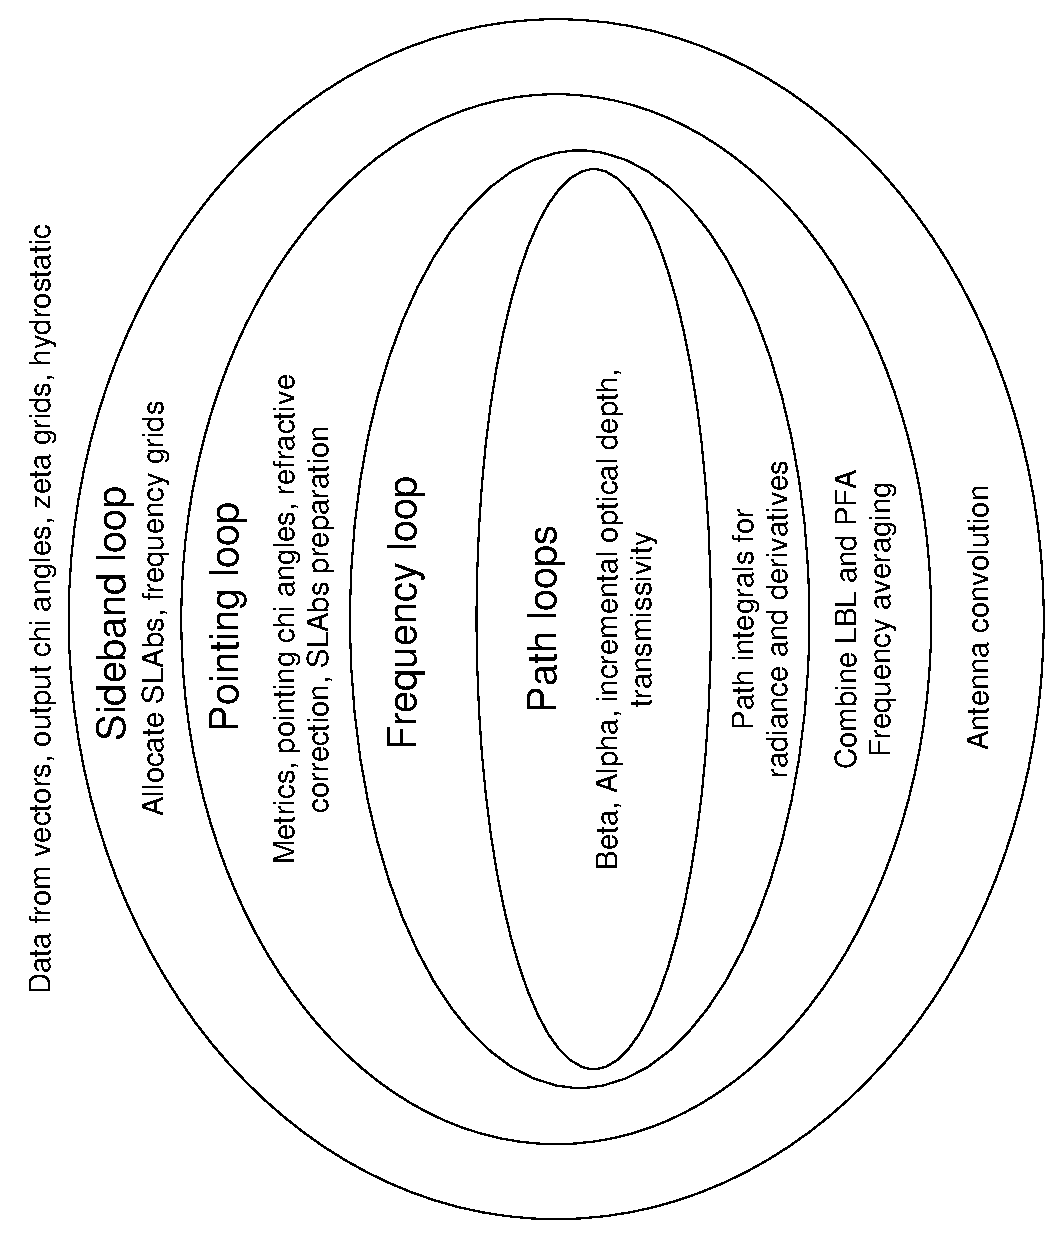
\includegraphics[scale=0.45,angle=270]{wvs-063-diag}
\hfill}

\end{frame}
%
% -----------------------------------------------------------------------------
%
\newframe{Data structures --- overview and arrays (1)}

Most of the data structures in the full forward model are arrays.  In
addition, the {\tt ForwardModelConfig\_T}, {\tt Grids\_T}, {\tt
Sparse\_t}, {\tt Vector\_T}, {\tt VectorValue\_T} structures, and others,
are used. The {\tt Sparse\_t}, {\tt Vector\_T} and {\tt VectorValue\_T}
structures are not further described here.

\vspace*{5pt}
$\zeta \times \phi$ arrays, where $\phi$ is the horizontal representation
basis for temperature and $\zeta$ is the union of $\zeta$ grids for all
interesting species, plus intermediate $\zeta$ values for Gauss-Legendre
quadrature, represent quantities at reference $\zeta$ and $\phi$ values
along the line of sight.

\end{frame}
%
% -----------------------------------------------------------------------------
%
\newframe{Data structures --- overview and arrays (2)}

Path arrays represent ``boundary'' quantities and ``layer'' quantities.

\vspace*{5pt}
Boundary quantities are those whose values are assumed to be on a
constant-$\zeta$ surface, such as temperature.

\vspace*{5pt}
Layer quantities represent quantities computed as an integral across a
layer between two constant-$\zeta$ surfaces, such as incremental optical
depth.

\vspace*{5pt}
In addition, path quantities are represented on a ``coarse'' grid
consisting of $\zeta$ values specified in the configuration (and a few
others that metrics calculations might add), and a ``fine'' grid
consisting of Gauss-Legendre (GL) points inserted to allow higher-accuracy
line-of-sight integration.

\end{frame}
%
% -----------------------------------------------------------------------------
%
\newframe{Data structures --- more arrays}

Derivatives are Path $\times$ State Vector quantities.  Some of these use
the same representation as used for interpolation coefficients, which are
sparse because we use bilinear interpolation.  Interpolation coefficients
are used for the chain rule.

\vspace*{5pt}
Derivatives and related quantities were originally represented by Path
$\times$ Species arrays.  Just filling them with zeros was taking 15\% of
our run time!

\vspace*{5pt}
The sparse representation for interpolation coefficients, using the {\tt
Sparse\_t} structure, is described in wvs-151.

\end{frame}
%
% -----------------------------------------------------------------------------
%
\newframe{Data structures --- Configuration}

The {\tt ForwardModelConfig\_T} structure specifies

\begin{itemize}

\item for which species and signals the forward model is to be evaluated,

\item whether line-by-line (LBL) or pre-frequency-averaged (PFA)
 calculations are to be done for specified species and signals, and

\item numerous options, such as whether temperature
derivatives are to be evaluated.

\end{itemize}

Part of this data structure is created when the L2CF is analyzed, and part
of it is created and destroyed upon each invocation of and return from the
full forward model.  The latter part isn't used by other models, such as
the quasi-linear model, the cloud model, the scan model.

\end{frame}
%
% -----------------------------------------------------------------------------
%
\newframe{Data structures --- {\tt Grids\_T} (1)}

The {\tt Grids\_T} structure represents

\begin{itemize}

\item co\"ordinates

 \begin{itemize}
 \item $f$ (frequency),
 \item $\zeta$ (- $\log_{10} P$),
 \item $\phi$ (orbit angle, measured from the equator on the ascending
   part of the orbit), and
 \item across the viewing plane (for the magnetic field), and
 \end{itemize}

\item values on grids having those co\"ordinates, for one or more species
 from the state or extra vectors.

\end{itemize}

The co\"ordinate grids, and indeed whether a dimension is present, can be
different for each species, so this is a complicated structure.

\end{frame}
%
% -----------------------------------------------------------------------------
%
\newframe{Data structures --- {\tt Grids\_T} (2)}

\begin{centering}
\bfseries\large Same structure for $f$, $\phi$, $\zeta$, \emph{cross}
grids, and data values\\
\includegraphics[width=2.15in,height=3.15in,angle=270]{wvs-063-grids_t}\\
\end{centering}

2-, 3-, or 4-d arrays of data values are stored in column-major order ($f
\times \zeta \times \phi\, \times\,$\emph{cross}) in a 1-d array.  Explicit
multidimensional subscript calculations are necessary (using support
routines in {\tt mlspgs/lib/Array\_stuff}).

\end{frame}
%
% -----------------------------------------------------------------------------
%
\newframe{Overview of {\tt FullForwardModel\_m}}

The {\tt FullForwardModel\_m} module has two module procedures, a public
one and a private one.

\vspace*{5pt}
The public one is {\tt FullForwardModel}.  It computes a reference $\zeta$
grid that consists of the union of the $\zeta$ grids for all species
specified in the configuration, plus intermediate $\zeta$ values for
Gauss-Legendre quadrature.  A configuration option allows oversampling
this grid.  Then it computes the sizes of numerous arrays, which in some
cases requires getting data from various sources.

\vspace*{5pt}
{\tt FullForwardModel} then calls {\tt FullForwardModelAuto}, which does
the real work.  {\tt FullForwardModelAuto} has numerous automatic arrays,
which avoids explicit allocation.  This makes the code somewhat smaller,
makes it impossible to forget deallocation, and, for some compilers, might
be more efficient than explicit allocation.

\end{frame}
%
% -----------------------------------------------------------------------------
%
\newframe{{\tt FullForwardModelAuto}}

{\tt FullForwardModelAuto} does some initialization, then the sideband
loop, then some cleaning up.

\vspace*{5pt}
First it references the subroutine {\tt Both\_Sidebands\_Setup} to get
quantities from the state vector or extra vector, to compute output $\chi$
angles, and to compute the integration $\zeta$ grid from the $\zeta$
reference grid by inserting points needed for Gauss-Legendre integration.

\vspace*{5pt}
Then it uses {\tt Two\_d\_Hydrostatic} to compute height and some
derivatives of height with respect to temperature and $\zeta$ on $\zeta
\times \phi$ grids, given temperature on state-vector grids, where $\phi$
is the horizontal representation basis for temperature, and $\zeta$ is the
integration $\zeta$ grid.

\vspace*{5pt}
Cleaning up consists of some debug printing and deallocating the few
arrays that are explicitly allocated.

\end{frame}
%
% -----------------------------------------------------------------------------
%
\newframe{Sideband loop}

\vspace*{5pt}
The sideband loop uses {\tt AllocateSlabs} to allocate data structures --
mostly spectroscopy catalog extracts -- used for single-line absorption
(SLAbs) calculations.

\vspace*{5pt}
Then it calls the internal subroutine {\tt Frequency\_Setup\_1} to work
out which frequency grids to use.  {\tt Frequency\_Setup\_1} has separate
parts for frequency averaging and monochromatic runs.

\vspace*{5pt}
Then it runs the pointing loop, which calls the internal subroutine {\tt
One\_Pointing}.  A ``pointing'' isn't a MIF.  It is a line of sight that
is tangent at one of the reference $\zeta$'s.  The $\zeta$'s along that
line are initially the subset of the integration $\zeta$'s from the
tangent upwards;  metrics calculations might add some $\zeta$'s.

After the pointing loop, the sideband loop calls the internal subroutine
{\tt Convolution}, which either does antenna convolution, or interpolates
to PTan.

\end{frame}
%
% -----------------------------------------------------------------------------
%
\newframe{Pointing loop (1)}

The body of the pointing loop is the {\tt One\_Pointing} internal
subroutine. It consists of

\begin{enumerate}

\item Calling {\tt Frequency\_Setup\_2} to get the frequencies needed for
  the current pointing (before {\tt One\_Pointing})

\item Setup

\item Metrics calculations

\item More setup that depends on metrics

\item Getting the magnetic field on the path if necessary

\item Computing interpolating coefficients $\eta^k_i(s)$ for species that
  do not depend upon frequency

\item Using $\eta^k_i(s)$ to interpolate mixing ratios from {\tt Grids\_T}
  to the line-of-sight path giving $f^k_i(s)$, for species that do not
  depend upon frequency

\item Computing pointing $\chi$ angles

\end{enumerate}
\dots

\end{frame}
%
% -----------------------------------------------------------------------------
%
\newframe{Equivalent Circular Earth Geometry}

\vspace*{-8pt}
\hfill
\includegraphics[angle=270,scale=0.475]{wvs-063-eq-circ}
\hfill

\end{frame}
%
% -----------------------------------------------------------------------------
%
\newframe{Pointing loop (2)}

\dots
\begin{enumerate}
\setcounter{enumi}{8}

\item Computing refractive correction using the subroutine {\tt
 Comp\_Refcor}

\item SLAbs preparation using {\tt Get\_GL\_SLabs\_Arrays}

\item Executing the frequency loop, which consists of calling the internal
 subroutine {\tt One\_Frequency} to do the radiative transfer for all LBL
 species (if any),

\item Frequency averaging the LBL radiance and derivatives at each point
 on the integration path, if there are any PFA species,

\item Calling {\tt One\_Frequency} again to do the radiative transfer for
 PFA species (if any),

\item Combining LBL and PFA results

\item Either doing frequency averaging using the filter shapes, or just
 storing the result of monochromatic or pure PFA (no LBL molecules)
 calculations.

\end{enumerate}

\end{frame}
%
% -----------------------------------------------------------------------------
%
\newframe{Metrics (1)}

Metrics calculations are done in several steps
\begin{enumerate}

\item The subroutine {\tt Tangent\_Metrics} calculates the equivalent
 earth radius at the tangent point, the height of the first $\zeta$
 (usually 1000 mb) reference surface, the height of the tangent point, and
 the subset of integration grid $\zeta$'s that are above the tangent and
 therefore along the line of sight.\\[5pt]

 For an Earth-intersecting pointing, the ``tangent point'' is actually
 the reflection point, and $\zeta$'s below the Earth surface defining the
 pointing direction.

\item Hydrostatic calculations are repeated to get a new $\zeta\times\phi$
 height reference grid if $\zeta$'s change because the pointing results in
 an earth-intersecting ray.

\item The subroutine {\tt Height\_Metrics} calculates $H$ and $\phi$ for
 the intersections of the line of sight with the integration grid
 $\zeta$'s.

\end{enumerate}

\dots

\end{frame}
%
% -----------------------------------------------------------------------------
%
\newframe{Metrics --- {\tt Height\_Metrics}}

\begin{multicols}{2}
\small

{\tt Height\_Metrics} uses a Newton iteration in $\phi \times h$ Cartesian
co\"ordinates, not polar co\"ordinates, to solve for the intersections of
the red and green lines (see wvs-048).

\vspace*{5pt}
Green lines are the heights of surfaces of constant $\zeta$, represented as
piecewise-linear segments by the $\zeta\times\phi$ height reference array
{\tt h\_glgrid}, which was computed by {\tt two\_d\_hydrostatic}.

\vspace*{5pt}
Red lines are the line of sight -- represented by the secant curve $H =
H_t \sec \delta\phi$, where $\delta\phi = \phi - \phi_t$.\\[-1pt]

\vspace*{-0.2in}
{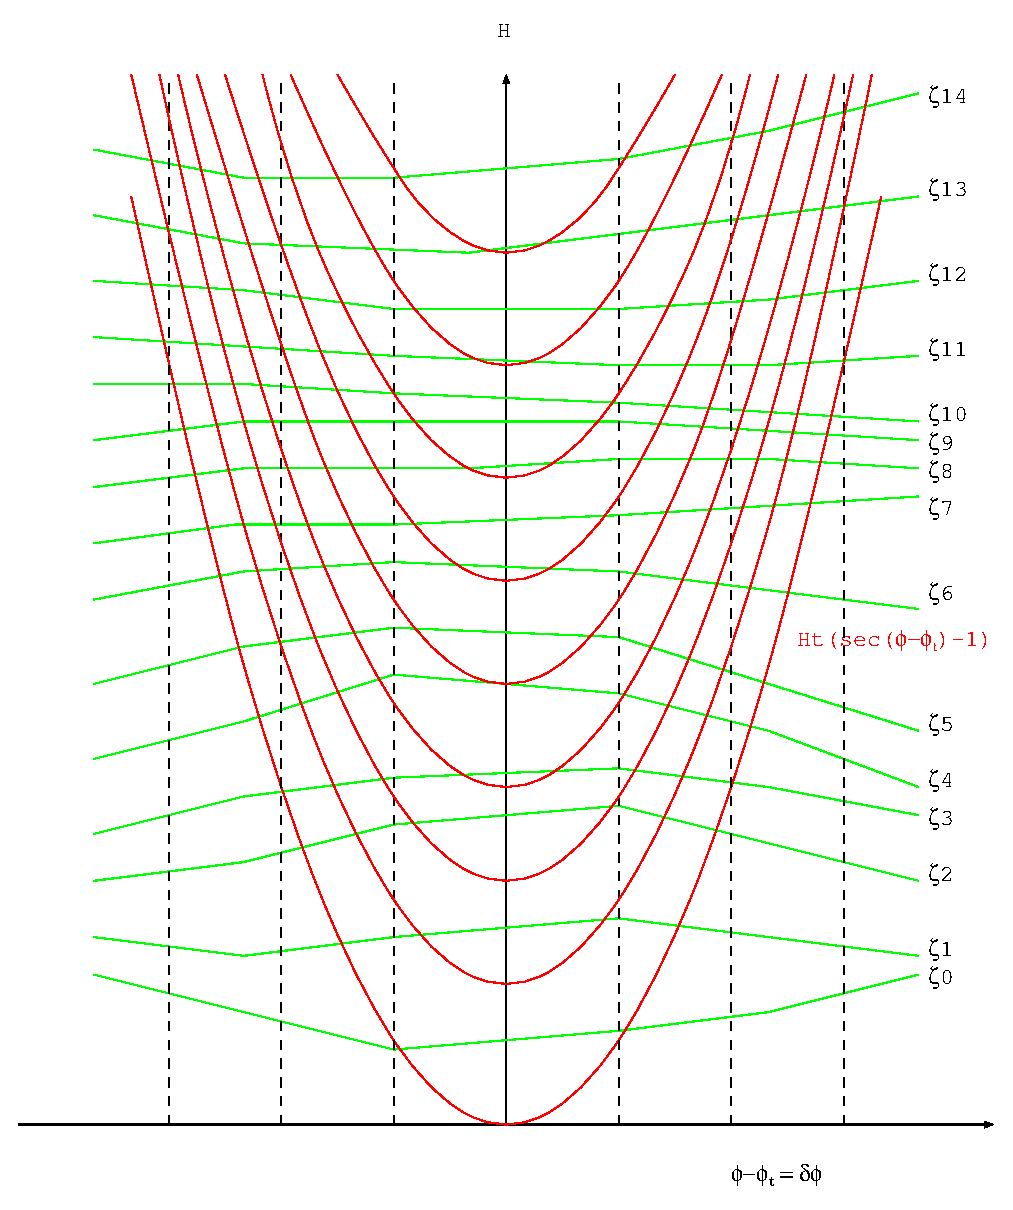
\includegraphics[width=2.25in,height=2.8125in]{wvs-048-grid2}}\\

\end{multicols}

\end{frame}
%
% -----------------------------------------------------------------------------
%
\newframe{Metrics (aside)}

Rather than solving for the intersection of the path represented by $H =
H_t \sec \delta\phi$ with piecewise-planar height surfaces, the QTM
model approximates the heights of constant-pressure surfaces as segments
of a sphere, each defined by the vertices of a facet, and the radius of
curvature of the equivalent circular Earth at the centroid of the facet
plus the average height of the facet's vertices (see wvs-132).  It then
calculates the intersections of the straight-line path with those
surfaces (see wvs-141).

\vspace*{5pt}
The same scheme could be used in the two-dimensional model by
approximating the heights of constant-pressure surfaces as segments of
circles. The resulting metrics calculation would be much simpler -- a
geometric calculation instead of a Newton iteration -- but would produce
very slightly different results.

\end{frame}
%
% -----------------------------------------------------------------------------
%
\newframe{Metrics (2)}

\begin{enumerate}
\setcounter{enumi}{3}

\item The subroutines {\tt More\_Points}, {\tt Min\_Zeta} and {\tt
 Add\_Points} might add $\zeta$'s in addition to the ones identified by
 {\tt Tangent\_Metrics}.

 (This step might actually be disabled in the code.)

\item The subroutine {\tt Compute\_GL\_Grid} inserts $\zeta$ points along
 the line of sight for Gauss-Legendre integration -- postponed until now
 because {\tt Add\_Points} might add some.

\item The subroutine {\tt More\_Metrics} calculates temperature $T_i(s)$,
 geometry-related derivatives along the line of sight, including at the GL
 points, $\frac{\d h_i(s)}{\d \zeta}$, temperature interpolation
 coefficients $\eta^T_i(s)$, \dots.

\end{enumerate}

\end{frame}
%
% -----------------------------------------------------------------------------
%
\newframe{SLAbs Preparation}

SLAbs (Single Line Absorption) preparation consists of filling the
structures allocated by {\tt AllocateSlabs} with values that depend upon
the spectroscopic parameters for each relevant line, and the temperature
and pressure at the points along the line of sight computed by the Metrics
calculations, but not those that depend upon frequency.  This is
ultimately done either by {\tt Slabs\_Prep} or {\tt Slabs\_Prep\_dT},
depending upon whether temperature derivatives are requested.  The
computed quantities are

\begin{itemize}

\item $\nu_{0_s}$, the pressure- and doppler-shifted line center (MHz),

\item $x_1$, the Doppler half-width (MHz),

\item $y$, collision width / Doppler half-width (MHz),

\item $y_i$, interference contribution,

\item {\tt Slabs1}, frequency-independent part of {\tt Slabs},

\item $\frac{\text{d {\tt Slabs1}}}{\text{d} \nu_0}$,

\item $\frac{\text{d}\nu_{0_s}}{\text{d}T}$,
 $\frac{\text{d}x_1}{\text{d}T}$, $\frac{\text{d}y}{\text{d}T}$,
 $\frac{\text{d}y_i}{\text{d}T}$,  and $\frac{\text{d}{\text{\tt
 Slabs1}}}{\text{d}T}$ if temperature derivatives are requested.

\end{itemize}

\end{frame}
%
% -----------------------------------------------------------------------------
%
\newframe{Frequency loop --- overview}

\small
The body of the frequency loop, in the internal subroutine {\tt
One\_Frequency}, does the radiative transfer for each requested
frequency.  Frequencies are either from the pointing frequency grid (for
the LBL frequency-averaging case), or the channel centers (for
monochromatic or PFA calculations). The steps for each frequency are

\small
\begin{enumerate}
\itemsep -1pt

\item Interpolate mixing ratios from {\tt Grids\_T} to the line-of-sight
 path giving $f^k_i$, for species (extinction) that depend upon frequency.

\item Evaluate $\beta^k_i$ and $\alpha_i = \sum_k f^k_i \beta^k_i$ for
 each species $k$ and each point $i$ on the coarse path, and incremental
 optical depth $\Delta\delta_{i \rightarrow i-1}$, for each layer, using a
 rectangular quadrature formula.

\item Call {\tt Path\_Contrib} to determine where GL is needed, using
 $\Delta\tau_i$.

\item Where GL is not needed, replace $\Delta\delta_{i \rightarrow i-1}$
 by a trapezoidal estimate.

\item Evaluate $\beta^k_i$ and $\alpha_i$ for GL, and $\Delta\delta_{i
 \rightarrow i-1}$ using GL, where necessary.

\item Compute $\tau_i = \exp\left(-\sum_{j=2}^i \Delta\delta_{j
 \rightarrow j-1}\right) \approx \exp \left( -\int_{\zeta_1}^{\zeta_i}
 \alpha(\zeta) \, \text{d} \zeta \right)$.

\item Compute radiance $I = \sum_{i \in \text{layers}} \Delta B_i \tau_i$,
 where $B_i = \frac{h \nu}{k \left(\exp\left(\frac{h \nu}{k
 T_i}\right)-1\right)}$ is the Planck function.

\item Compute derivatives $\frac{\partial I}{\partial T_i}$ and
 $\frac{\partial I}{\partial f^k_i}$ ($f^k_i$ is mixing ratio for
 $k^\text{th}$ species).

\end{enumerate}

\end{frame}
%
% -----------------------------------------------------------------------------
%
\newframe{Frequency loop --- $\beta$ and $\alpha$}

For each frequency and species, $\beta^k_i$ is computed using a method
that depends upon whether the calculation is LBL or PFA, scalar or
polarized, or cloudy.

\begin{itemize}
\item {\tt Get\_Beta\_Path} for scalar LBL
\item {\tt Get\_Beta\_Path\_PFA} for scalar PFA
\item {\tt Get\_Beta\_Path\_Polarized} for Polarized (which can't be PFA)
\item {\tt Get\_Beta\_Path\_Cloud} for clouds (also not PFA)
\end{itemize}

$\alpha_i = \sum_{k \in \text{species}} f^k_i \beta^k_i$, where $f^k_i$ is
the mixing ratio of the $k^{\text{th}}$ species at the $i^{\text{th}}$
point along the line of sight.  For GL calculations, $\alpha_{ij} =
\sum_{k \in \text{species}} f^k_{ij} \beta^k_{ij}$, where $j$ indexes the
GL point in the $i^{\text{th}}$ layer.

\end{frame}
%
% -----------------------------------------------------------------------------
%
\newframe{Frequency loop --- $\Delta\delta_{i \rightarrow i-1}$ and $\tau_i$}

\small

The incremental optical depth $\Delta\delta_{i \rightarrow i-1} =
\int_{s_i}^{s_{i-1}} \alpha_i\, \text{d} s$.  The contribution from the
$k^\text{th}$ species is $\Delta\delta^k_{i \rightarrow i-1} =
\int_{s_i}^{s_{i-1}} f^k_i(s) \beta^k_i\, \text{d} s$.

Where GL is needed, these are computed in $\zeta$ co\"ordinates, \emph{viz.}
$\Delta\delta_{i \rightarrow i-1} \!\approx\! \sum_{j=1}^{N_{\text{GL}}}
\omega_j \left(\alpha \frac{\text{d}s}{\text{d}h}
\frac{\text{d}h}{\text{d}\zeta} \right)_{ij} \Delta\zeta $
%= \int_{\zeta_i}^{\zeta_{i-1}} \alpha_{ij} \frac{\text{d}s}{\text{d}h}
%\frac{\text{d}h}{\text{d}\zeta} \text{d} \zeta $
and
$\Delta\delta^k_{i \rightarrow i-1}
\!\approx\! \sum_{j=1}^{N_{\text{GL}}} \omega_j \left( f^k \beta^k
\frac{\text{d}s}{\text{d}h} \frac{\text{d}h}{\text{d}\zeta} \right)_{ij}
\Delta\zeta $.\\
%= \int_{\zeta_i}^{\zeta_{i-1}} f^k_{ij} \beta^k_{ij} \frac{\text{d}s}{\text{d}h}
%\frac{\text{d}h}{\text{d}\zeta} \text{d} \zeta$.\\
$s = \sqrt{h^2-h^2_t}$, so
$\frac{\text{d}s}{\text{d}h} = \frac{h}{\sqrt{h^2-h_t^2}}$, which is singular
at the tangent point $h = h_t$; this is partially canceled using the
rectangular estimate:\\
$\int_{\zeta_i}^{\zeta_{i-1}} G(\zeta) \frac{\text{d}s}{\text{d}h}
 \frac{\text{d}h}{\text{d}\zeta}\, \text{d} \zeta =
G(\zeta_i) \int_{\zeta_i}^{\zeta_{i-1}} \frac{\text{d}s}{\text{d}h}
 \frac{\text{d}h}{\text{d}\zeta}\, \text{d} \zeta +
 \int_{\zeta_i}^{\zeta_{i-1}} \left[G(\zeta)-G(\zeta_i)\right]
 \frac{\text{d}s}{\text{d}h}
 \frac{\text{d}h}{\text{d}\zeta}\, \text{d} \zeta$.\\
The first integral on the right is just $\Delta s_{i \rightarrow i-1}$, so
the first term on the right is the rectangular estimate. 
$G(\zeta)-G(\zeta_i) = 0$ for $\zeta = \zeta_i$, which cancels the
singularity in $\frac{\text{d}s}{\text{d}h}$ at the tangent point if
$\zeta_i = \zeta_t$.

Transmissivity $\tau_i = \exp \left( - \sum_{j=2}^i \Delta\delta_{i
\rightarrow i-1} \right)$.  The running sum of $\Delta \delta_{i
\rightarrow i-1}$ is only taken until it exceeds $\ln \Omega$, using the
rectangular quadrature estimate, where $\Omega$ is the largest
floating-point number, after which {\tt exp} underflows, so $\tau_i = 0$
thereafter.

\end{frame}
%
% -----------------------------------------------------------------------------
%
\newframe{Frequency loop (aside) }

$\beta^k_i$ and $\Delta\delta_{i \rightarrow i-1}$ are initially computed
for all boundaries and layers on the integration path.

Then the ``black out'' position on the path (where $\tau_i$ underflows) is
computed.

Computing $\beta^k_i$ is the single most-expensive thing the full forward
model does.  If $\beta^k_i$ and $\Delta\delta_{i \rightarrow i-1}$ were
computed one layer at a time, it would not be necessary to compute them
after the ``black out'' position.

``Black out'' occurs on the lowest-pointing paths, which are also the
longest paths.  Not computing $\beta^k_i$ beyond the ``black out''
position might result in significant performance improvement -- but this
would require significant re-organization of {\tt One\_Frequency}.

\end{frame}
%
% -----------------------------------------------------------------------------
%
\newframe{Frequency loop --- Mixing Ratio Derivatives }

$\frac{\partial I}{\partial f^k_i}$ is computed by {\tt DRad\_Tran\_df}
from the {\tt Rad\_Tran} module.  This is a fairly straight-forward
computation consisting of the following steps:

\begin{enumerate}

\item Derivatives are evaluated using rectangular quadrature to
approximate $\frac{\partial \Delta\delta_{s_{i-1} \rightarrow s_i}}
                  {\partial f^k} =
\int_{s_{i-1}}^{s_i} \frac{\partial \alpha(s)}{\partial f^k}\, \d s$.

\item Where the radiance path integration needed GL improvement, the
 derivatives are improved using GL.

\item The refractive correction is applied.

\item Individual integrals are summed using Equations (10.7-9) from the
 ATBD, using {\tt Dscrt\_dx} from the {\tt Scrt\_dn\_m} module.

\end{enumerate}

Notice that for mixing ratio derivatives $\frac{\partial \Delta
B_i}{\partial f^k_i}$ is zero.

\end{frame}
%
% -----------------------------------------------------------------------------
%
\newframe{Frequency loop --- Temperature Derivatives }

$\frac{\partial I}{\partial T_i}$ is computed by {\tt DRad\_Tran\_dT}. 
This is similar in broad outline to {\tt DRad\_Tran\_df} but is
significantly complicated by the need to take into account the derivatives
of height w.r.t.\ temperature, because the path in $\zeta$ co\"ordinates
depends upon temperature.  At the end the individual integrals are summed
using {\tt Dscrt\_dT}.  $\frac{\partial \Delta B_i}{\partial T_i}$ is not
zero.

\end{frame}
%
% -----------------------------------------------------------------------------
%
\newframe{Pointing loop --- Frequency averaging}

If a configuration requests frequency averaging, has both LBL and PFA
$\beta$'s, and requests derivatives, some preliminary work on frequency
averaging is done by the internal subroutines {\tt
Frequency\_Avg\_Rad\_Path} and {\tt Frequency\_Average\_Derivatives},
which in turn uses {\tt Fre\-quen\-cy\_\-Average\_Derivative}.

\vspace*{5pt}
Then the internal subroutine {\tt Frequency\_Average} is used either to
average using the filter shapes, or just to store the result for
monochromatic runs. {\tt Fre\-quency\_Average} uses {\tt SCRT\_PFA} from
the {\tt Scrt\_dn\_m} module to combine $\tau_i$ for LBL and PFA
molecules.

\vspace*{5pt}
{\tt Fre\-quen\-cy\_\-Average\_Derivative} and {\tt Frequency\_Average}
use the subroutines {\tt Freq\_Avg} and {\tt Freq\_Avg\_DACS} from the
{\tt Freq\_Avg\_m} module.

\end{frame}
%
% -----------------------------------------------------------------------------
%
\newframe{Pointing loop --- Frequency averaging (cont.)}

The subroutine {\tt Freq\_Avg}

\begin{enumerate}

\item Uses {\tt Freq\_Avg\_Setup} to find the positions in the pointing
 frequency grid of the minimum and maximum frequency in the filter shape
 table.

\item Uses {\tt Freq\_Avg\_Avg} to fit the radiances or derivatives, as a
 function of frequency, with a spline.

\item Evaluates the spline at the frequencies of the filter shape grid.

\item Multiplies the interpolated radiance or derivative by the frequency
 response.

\item Integrates the product using Simpson's rule or the Newton-Cotes 3/8
 rule.

\end{enumerate}

The subroutine {\tt Freq\_Avg\_DACS} uses the Math77 subroutine {\tt
DTCST} to convolve DACS radiances or derivatives with the filter, using a
Fourier cosine-sine transform. More modern software, e.g., {\tt FFTW},
would be faster, but the transforms are small, and {\tt mlsl2} doesn't
spend much time here.

\end{frame}
%
% -----------------------------------------------------------------------------
%
\newframe{Pointing loop --- Frequency averaging (aside)}

Since frequency averaging uses only radiances and derivatives calculated
for frequencies within the range of the filter shape, the radiative
transfer calculation need not be performed for frequencies outside this
range.  But it is.

\end{frame}
%
% -----------------------------------------------------------------------------
%
\newframe{Pointing loop --- PFA}

The frequency loop is run separately, first for LBL species (if any) and
then for PFA species (if any). If there are any PFA species, the radiances
from LBL species will have been separately frequency averaged at every
point on the path.

\vspace*{3pt}
PFA $\beta^k_i$ is obtained by interpolation in PFA ($T \times P$) tables
instead of spectroscopic modeling.  PFA tables are computed offline by
special runs of {\tt mlsl2}.

\vspace*{3pt}
$\tau_i$ for PFA is multiplied by the frequency-averaged $\tau_i$ from the
LBL calculation, and the product integrated to give combined LBL and PFA
transmittance for the channel.  See wvs-028 and its references.

\vspace*{3pt}
Temperature derivatives are computed as if they were mixing-ratio
derivatives, to avoid including the Planck function derivative
$\frac{\partial \Delta B_i}{\partial T_i}$ and hydrostatic effects twice.

\vspace*{3pt}
LBL and PFA derivatives are simply added during the frequency-averaging step.

\end{frame}
%
% -----------------------------------------------------------------------------
%
\newframe{Sideband loop --- Antenna convolution}

The internal subroutine {\tt Convolution} either convolves the radiances
and derivatives from all the pointings with the antenna pattern, or just
interpolates them to PTan, using the following steps:

\begin{enumerate}

\item It makes sure the pointing $\chi$ angles are strictly increasing,
 and patches them in an ad-hoc way if not.

\item It works out which antenna pattern to use, and applies the elevation
 offset.

\item It uses {\tt FOV\_Convolve\_Setup} from the {\tt FOV\_Convolve\_m}
 module to fill the {\tt Convolve\_Support} structure with data that
 depend only on pointing $\chi$ angles.

\end{enumerate}

\end{frame}
%
% -----------------------------------------------------------------------------
%
\newframe{Sideband loop --- Antenna convolution (cont.)}

\small
Using the {\tt Convolve\_Support} structure, the radiances are convolved
using the following subroutines from the {\tt Convolve\_All\_m} module:

\begin{itemize}
\itemsep -1pt

\item {\tt Convolve\_Radiance} for radiances.

\item {\tt Convolve\_Temperature\_Deriv} for temperature derivatives.  The
 temperature derivative also includes hydrostatic contributions that model
 the effect of a temperature change on the antenna pattern that is
 remapped onto $\zeta$ co\"ordinates.

\item {\tt Convolve\_Other\_Deriv} for mixing-ratio or
spectroscopy-parameter. derivatives

\end{itemize}

The subroutine {\tt Convolve\_Radiance} uses the subroutine {\tt
FOV\_Con\-volve\_\-1d} from the module {\tt FOV\_Convolve\_m}.  The
subroutine {\tt Con\-volve\_\-Tem\-perature\_Deriv} uses the subroutine
{\tt FOV\_Con\-volve\_\-Temp\_Derivs}.  The subroutine {\tt
Convolve\_Other\_Deriv} uses the subroutine {\tt FOV\_Convolve\_2d}.

The subroutines in the module {\tt FOV\_Convolve\_m} use the Math77
subroutines {\tt DTCST} to compute a cosine transform, and {\tt DRFT1} to
compute a full FFT.

\end{frame}
%
% -----------------------------------------------------------------------------
%
\newframe{Sideband loop --- No antenna convolution}

If antenna convolution is not requested, the subroutine {\tt
Inter\-po\-late\_\-Array\_Setup} from the module {\tt MLSNumerics} is
used.  Then the following subroutines from the module {\tt
Convolve\_All\_m} are used:

\begin{itemize}

\item {\tt Interpolate\_Radiance} to interpolate radiance

\item {\tt Interpolate\_Temperature\_Deriv} to interpolate temperature
 derivatives

\item {\tt Interpolate\_Other\_Deriv} to interpolate mixing-ratio and
 spectroscopy-parameter derivatives

\end{itemize}

\end{frame}
%
% -----------------------------------------------------------------------------
%
\newframe{Sideband loop --- Cleaning up}

After interpolation to PTan (but not after convolution), if the {\tt l2cf}
field {\tt ScanAverage} in the forward model configuration is true, the
subroutines {\tt ScanAverage\_1d} and {\tt ScanAverage\_2d} from the
module {\tt ScanAverage\_m} are used to average the radiances and
derivatives, respectively, from the pointing $\chi$ angles to the MIF
$\chi$ angles, to take motion during the MIF into account.

\vspace*{5pt}
The subroutine {\tt Interpolate\_Values} is used to interpolate radiances
and derivatives for each pointing to eight-point GL grids between each
pair of values from the {\tt MIF\_Times} grid (quantity type {\tt
L1bMIF\_TAI}).  Those interpolated values are then integrated to the {\tt
MIF\_Times} grid using an eight-point Gauss-Legendre quadrature.

\vspace*{5pt}
Finally, some arrays explicitly allocated in {\tt FullForwardModelAuto}
are deallocated, and some debug printing is done if requested.

\end{frame}
%
% -----------------------------------------------------------------------------
%
\newframe{References (1)}

\small
The primary reference is the Full Forward Model ATBD, JPL D-18130.

\vspace*{5pt}
Many of the modules have embedded \LaTeX-isms, and can be turned into
\LaTeX\ files from which nice listings with typeset mathematics can be
produced by using my $\sim${\tt vsnyder/progs/f90tex} program (also in
{\tt mlspgs/util}).

\vspace*{5pt}
Several of my memos (in {\tt mlspgs/doc/}) might be helpful:

\begin{itemize}
\item wvs-017: Pre-frequency averaging
\item wvs-018: Temperature derivatives
\item wvs-019: Betas, {\tt slabs\_sw\_m}
\item wvs-022: Spectroscopy derivatives
\item wvs-024: PFA derivatives
\item wvs-025: New frequency averaging scheme for use with PFA
\end{itemize}
\end{frame}
%
% -----------------------------------------------------------------------------
%
\newframe{References (2)}

\begin{itemize}
\item wvs-026: Simplifying assumption to combine line-by-line and PFA
\item wvs-027: Revised method to combine line-by-line and PFA
\item wvs-028: Summary of line-by-line and PFA radiance and derivatives
\item wvs-029: Refractive correction for $\phi$
\item wvs-033: Path integrations [a proposal, not a description]
\item wvs-037: Updated non-GL correction in forward model
\item wvs-038: Modification to {\tt metrics\_m}
\item wvs-039: Calculating $H_m$ in modification to {\tt metrics\_m}
\item wvs-040: Calculating $\phi$ for $\zeta_{\text{max}}$ [should be
$\zeta_{\text{min}}$]
\item wvs-041: Maximum [should be Minimum] $\zeta$
\item wvs-042: $H$--$\phi$ iteration in {\tt metrics}
\end{itemize}
\end{frame}
%
% -----------------------------------------------------------------------------
%
\newframe{References (3)}

\begin{itemize}
\item wvs-043: Inverting the $\phi$ refractive correction
\item wvs-044: What to do in {\tt metrics\_m}
\item wvs-046: Interesting result concerning $\zeta_{\text{min}}$
\item wvs-047: Revised metrics plan
\item wvs-048: Different solution for $\phi$--$H$ calculation in {\tt
 metrics\_m}
\item wvs-053: Alternative minimum $\zeta$ calculation
\item wvs-056: Refractive correction
\item wvs-059: Another look at metrics [turned out to be a bad idea]
\item wvs-060: Trouble with GL correction in the forward model
\item wvs-061: Trouble with path length in the forward model
\end{itemize}

\end{frame}
%
% ----------------------------------------------------------------------------
%
\end{document}

%%% Local Variables: 
%%% mode: latex
%%% TeX-master: t
%%% End: 

% $Log$
% Revision 1.11  2020/05/27 21:34:58  vsnyder
% Repair typo in equation on page 23
%
% Revision 1.9  2019/09/17 23:01:16  vsnyder
% Add comments about how to make the graphics
%
% Revision 1.8  2019/09/11 01:14:08  vsnyder
% Numerous improvements resulting from today's presentation
%
% Revision 1.7  2019/09/10 01:38:46  vsnyder
% Fix some typos, add some more explanation
%
% Revision 1.6  2019/09/04 00:13:27  vsnyder
% Correct page 14, add page 15
%
% Revision 1.5  2019/08/27 01:08:27  vsnyder
% Modest revisions and improvements
%
% Revision 1.4  2019/08/26 22:09:46  vsnyder
% Correct the date on the title page
%
% Revision 1.3  2019/05/31 17:17:21  pwagner
% A workaround for building beamerclass
%
% Revision 1.2  2019/05/23 00:26:28  vsnyder
% Convert to beamer class
%
% Revision 1.1  2008/06/11 20:14:54  vsnyder
% Initial commit
%
% Revision 1.1  2008/06/11 20:14:54  vsnyder
% Initial commit
%
% Revision 1.7  2001/06/16 00:57:56  vsnyder
% More stuff about least-squares, some clean-up
%
% $Id$
